\chapter{Método de trabajo}
\label{chap:metodo}

\section{Metodología de desarrollo}
En el apartado \ref{sec:3.2} se ha hablado de las metodologías de diseño de un sistema empotrado. Para realizar el diseño del sistema empotrado objetivo de este \acs{TFG} se debe diseñar el componente software de control, o firmware.\\

\subsection{Diseño basado en plataforma}
La metodología de desarrollo empleada para el desarrollo del sistema empotrado es el llamado <<Diseño basado en plataforma>>, donde los equipos de desarrollo del hardware y del software pueden trabajar de forma independiente y separados en el tiempo, o puede haber varios equipos de desarrollo software realizando diferentes sistemas sobre la misma placa hardware. En el artículo \cite{disPBD} se hace un pequeño repaso a cómo la utilización de los mismos componentes hardware reduce el coste global de desarrollo de varios sistemas empotrados con diferentes funcionalidades. Esta metodología tiene también sus inconvenientes ya que, al desarrollar el software de forma independiente, se pueden topar con restricciones que impidan continuar con el desarrollo y obliguen a rediseñar el sistema.\\

La metodología de desarrollo basada en plataforma permite de forma sencilla y barata desarrollar una <<familia de productos>> con componentes, módulos o subsistemas similares pero con tareas diferentes, pero el coste de organización empresarial y del portfolio del negocio se incrementa notablemente. A finales de los '90 IBM reorganizó sus equipos de desarrollo en torno a la idea de coordinar esfuerzos y poder reutilizar componentes desarrollados en una familia de productos bien planificada. Esto condujo a la reducción de entre un 70\% y 80\% de los módulos desarrollados y un ahorro de unos 700 Millones de \$ del coste de su estructura empresarial. Además de esto se incrementó el número de productos comercializados en un 270\%. En la Figura \ref{fig:IBMCost} podemos ver la evolución del ahorro de costes de IBM, el incremento del grado de reutilización y la opinión de sus trabajadores sobre el nuevo método de trabajo \cite{disPBD}.\\

\begin{figure}[!h]
\begin{center}
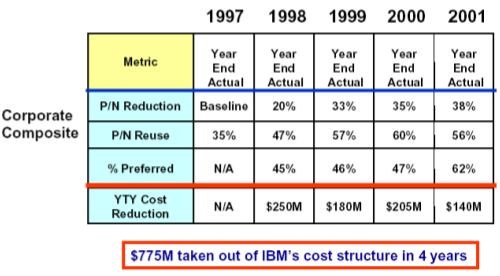
\includegraphics[width=0.7\textwidth]{figs/IBMCost.png}
\caption{Ahorro de costes en IBM después de aplicar el desarrollo basado en plataforma}
\label{fig:IBMCost}
\end{center}
\end{figure}

\subsection{Desarrollo guiado por pruebas}

Para la programación del firmware del sistema objetivo de este \acs{TFG} se utilizará la metodología de desarrollo guiado por pruebas, o TDD por sus siglas en inglés (Test-Driven Development). \\

El TDD involucra dos técnicas de programación: escribir las pruebas primero y refactorización después \cite{DesTDD}.\\

El proceso que se sigue es el siguiente: 
\begin{itemize}
\item En primer lugar se escribe una prueba y se verifica que falla.
\item A continuación, se implementa el código que hace que la prueba pase satisfactoriamente.
\item Seguidamente se refactoriza el código escrito.\\

\end{itemize} 
Podemos ver el flujo de trabajo en la figura \ref{fig:TDD}.\\

\begin{figure}[!h]
\begin{center}
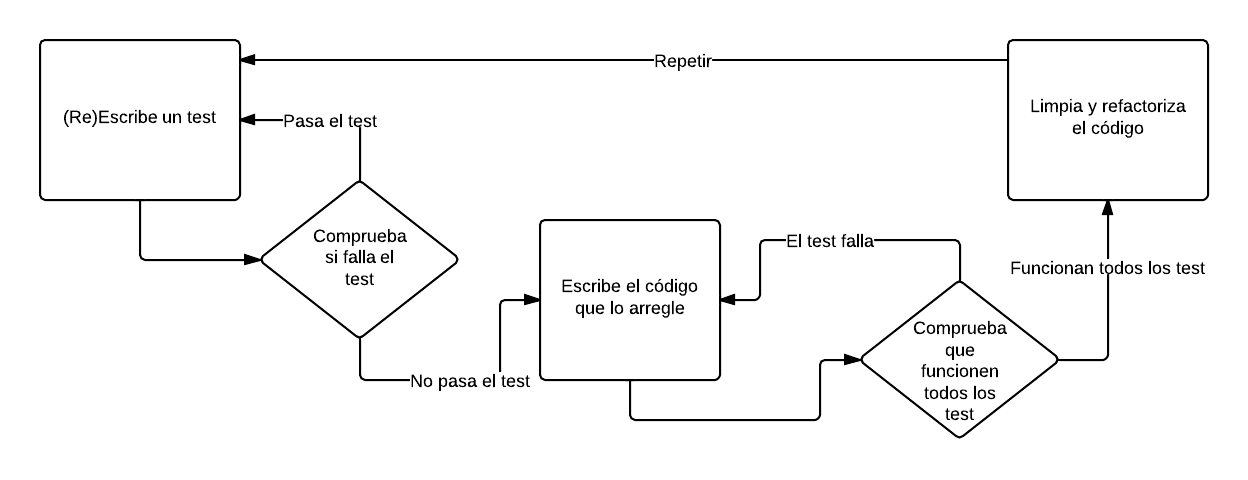
\includegraphics[width=1\textwidth]{figs/TDD.png}
\caption{Diagrama de flujo que define el funcionamiento del proceso de desarrollo orientado a test}
\label{fig:TDD}
\end{center}
\end{figure}


El propósito del desarrollo guiado por pruebas es lograr un código limpio que cumpla con la funcionalidad exigida. La idea es que los requisitos sean traducidos a pruebas, de este modo, cuando las pruebas pasen se garantizará que el software cumple con los requisitos que se han establecido \cite{DisAgilTDD}.\\

El motivo principal para utilizar TDD es la obligación de definir antes que nada la interfaz de comunicación entre componentes y su funcionalidad, además de tener un completo y creciente set de pruebas que permite asegurar que los componentes y funcionalidades testadas se realizan de forma correcta, y que siguen correctas en todo momento \cite{DisAgilTDD}.\\

Otro de los motivos es que al implementar única y exclusivamente el código necesario para hacer pasar los test se evita el escribir código innecesario, se reduce la redundancia de código y se eliminan los <<códigos muertos>> \cite{DisAgilTDD}, siendo esto último de especial importancia en sistemas con una fuerte restricción de memoria como es el sistema objetivo del proyecto. \\

Tener un completo set de pruebas en el desarrollo del software de un sistema empotrado es muy importante debido a la relativa inestabilidad de los prototipos utilizados, que pueden fallar total o parcialmente en un determinado momento, además de la práctica imposibilidad de aplicar parches al sistema una vez esté en producción.\\

La utilización del TDD en el desarrollo del sistema objetivo de este \acs{TFG} ha sido difícil teniendo en cuenta que no existe ningún entorno de desarrollo o \textit{framework} que facilite la tarea, así como tampoco existe ningún tipo de emulador de pruebas ni la capacidad del prototipo hardware de interactuar con el usuario fuera de la interfaz de programación. \\

La realización de las pruebas requeridas por la metodología de desarrollo se han realizado mediante funciones ejecutadas como si del sistema final se tratase. Para verificar si las pruebas han sido exitosas éstas funciones devuelven un número entero con un significado predefinido que indique el estado de éxito. Una vez las funciones han devuelto su estado de éxito la forma de comprobar cuáles son las pruebas que han tenido éxito y cuáles no s eha tenido que abrir una interfaz de depuración con \textit{gdb} y comprobar a mano los valores obtenidos.\\


\section{Tecnologías y herramientas utilizadas}
\label{tecUsadas}
En esta sección se comentan las herramientas hardware y software utilizadas durante la realización de este \acs{TFG}.\\

Para la realización del sistema propuesto se ha utilizado un prototipo hardware basado en la placa <<CPU ARM Cortex M3 STMF205VGT6>> y con el dispositivo GPS <<GlobalTop FGPMMOPA6H>> empotrado en la misma. Este prototipo no tiene ningún tipo de interfaz con el exterior que ayude a la interacción con el usuario, salvo la interfaz de programación y depuración.\\

La interfaz de programación y depuración utilizada para realizar este sistema ha sido un dispositivo comercial que ofrece la empresa que vende la placa, en concreto el dispositivo <<ST-Link/v2>>, que se comunica con la placa mediante comandos JTAG, un estándar de testing para placas definido en el estándar IEEE 1149.1.\\

En cuanto a los medios software empleados se ha utilizado el sistema operativo <<Ubuntu 12.04>>, el entorno de desarrollo <<Eclipse Kepler C/C++>> con los complementos <<GNU ARM toolchain>>, para la comunicación de Eclipse con el compilador cruzado <<Sourcery CodeBench>>, y <<Zylin Embedded CDT>> para comunicar Eclipse con el entorno de programación y depuración a través del programa <<OpenOCD>>.\\

Sobre las ayudas a la programación se disponen de las bibliotecas de funciones proporcionadas por el fabricante, el código fuente del sistema operativo FreeRTOS y mercurial para el control de versiones y la utilización de un repositorio en Bitbucket.\\


\subsection{Lenguaje de programación}
El lenguaje de programación con el que se realizará este \acs{TFG} es C, un lenguaje de alto nivel que nos permite también un control a muy bajo nivel e incluso programar algunas funciones en ensamblador si fuera necesario. Es el lenguaje en el que los fabricantes proporcionan las bibliotecas de funciones de sus componentes hardware.\\

El lenguaje C apareció en el mercado por primera vez en 1972 por Dennis Ritchie en los Laboratorios Bell y, pese a su antigüedad, sigue siendo uno de los lenguajes de programación más utilizados, pese a haber sufridos escasos cambios desde su nacimiento. Según un estudio de la compañía TIOBE Software el lenguaje C se sitúa en primera posición en cuanto al número de sistemas desarrollados en 2014 con un total del 16\% del total \cite{website:tiobe}.\\


